% TEMPLATE for Usenix papers, specifically to meet requirements of
%  USENIX '05
% originally a template for producing IEEE-format articles using LaTeX.
%   written by Matthew Ward, CS Department, Worcester Polytechnic Institute.
% adapted by David Beazley for his excellent SWIG paper in Proceedings,
%   Tcl 96
% turned into a smartass generic template by De Clarke, with thanks to
%   both the above pioneers
% use at your own risk.  Complaints to /dev/null.
% make it two column with no page numbering, default is 10 point

% Munged by Fred Douglis <douglis@research.att.com> 10/97 to separate
% the .sty file from the LaTeX source template, so that people can
% more easily include the .sty file into an existing document.  Also
% changed to more closely follow the style guidelines as represented
\section{Evaluation} \label{sec:eva}

We have implemented the proposed approach demonstrated in previous sections. The implementation modifies %$350$ SLoC to Linux kernel and $166$ SLoc to Xen hypervisor, of which $2$ SLoc in the hypervisor are 
$166$ SLoc of Xen hypervisor and $350$ SLoC of Linux kernel, which has efficiently improved the performance in page table management.

This section evaluates the performance of \name by running both micro- and macro-benchmark kits.

\subsection{Experimental Setup}

Our experimental platform is a LENOVO QiTianM4390 PC with Intel Core i5-3470 running at 3.20 GHz, four CPU cores available to the system. We enable the Intel VT-d feature in the BIOS menu, which supports queue-based invalidation interface in the granularity of page invalidation. Xen version 4.2.1 is used as the hypervisor while domain0 uses the Ubuntu version 12.04 and kernel version 3.2.0-rc1. In addition, domain 0 as the testing system configures its grub.conf to turn on I/O address translation for itself and to print log information to a serial port in debug mode.

Besides that, we have been aware that a process creation/exit will give rise to many page table updates (e.g., from a page of Writable to a page of Page Global Directory ), upon which function iotlb\_flush\_qi() will be invoked to flush corresponding IOTLB entries, and this is how a process-related operation affects IOTLB-flush. Thus, we place a global counter into the function body to log invocation times of the function and then an average counter per minute is calculated as a frequency of IOTLB-flush. When the recorded average counter drops to zero, it means that IOTLB-flush does not occur, indicating that no process is created or terminated then. In a nutshell, there exits a mutually positive effect between a process creation/exit and IOTLB-flush.

Because of that, we define two different settings, classified by the frequency of IOTLB-flush.

\emph{Idle-setting}: Actually, when system boots up and logins into graphical desktop, lots of system processes are created, causing many IOTLB flushes. But as time goes by, the frequency of IOTLB-flush reduces rapidly and stays stable to zero level ten minutes later, and we think that system starts to be in an idle setting, where no process creation/exit occurs and existing system daemons are still running.

\emph{Busy-setting}: We launch a stress tool emulating an update-intensive workload to transfer the system from the idle setting to a busy one. Specifically, the tool is busy periodically launching a default browser(e.g., Mozilla Firefox 31.0 in the experiment), opening new tabs one by one and then closing the browser gracefully in an infinite loop, so as to constantly create/terminate a large number of Firefox processes, thus giving rise to frequent page type updates of page tables. More precisely, one iteration of the loop costs five minutes and the frequency of process creation/termination are $542.14 times$ per minute and $542.07 times$ per minute, respectively. Besides, the memory usage of the tool on an average iteration is 284.1 MB. Please note that since the frequency of IOTLB-flush will become stable five minutes after the tool starts to run, time period of one iteration is also set to the time interval to achieve a stable flush frequency.

Since page tables do not update in the idle setting, our algorithm can not play a big role in system performance. Both micro- and macro-benchmark kits are performed under the busy setting, in which micro-tests are utilized to evaluate the frequency of IOTLB-flush, CPU usage and memory size while macro-benchmarks give an assessment on overall system performance.

\subsection{Micro-Benchmarks}

To begin with, micro-experiments are conducted in two groups. In one group called cache-disabled, the "idle" system enters into the busy setting without the cache pool enabled. On the contrary, system state changes in another cache-pre-enabled group where the tool is invoked when the cache is already enabled since system begins to run.

\begin{figure}[ht]
\centering
%\includegraphics[scale=0.55]{image/iotlbflush.png} \\
\includegraphics[width=0.5\textwidth]{image/micro/iotlbflush.png} \\
\caption{Frequency of IOTLB-flush drops sharply to zero whenever the page-table cache is enabled}
\label{fig:iotlbflush}
\end{figure}

As can be seen from figure\ref{fig:iotlbflush}. Y-axis represents the frequency of IOTLB-flush, corresponding to the time interval (i.e., one minute) of x-axis for the first thirty minutes that the running tool has taken up. From this figure, frequency in the cache-disabled group increases rapidly and remains stable five minutes later. By contrast, frequency in the cache-pre-enabled group drops to zero in a very short time and keeps zero level from then on. It can be safely concluded that our proposed algorithm does have a positive effect on reducing IOTLB frequency to zero quickly.

%\begin{figure*}[!t]
%\centering
%\subfigure[PGD Alloc]{
%\label{fig:subfig:a}
%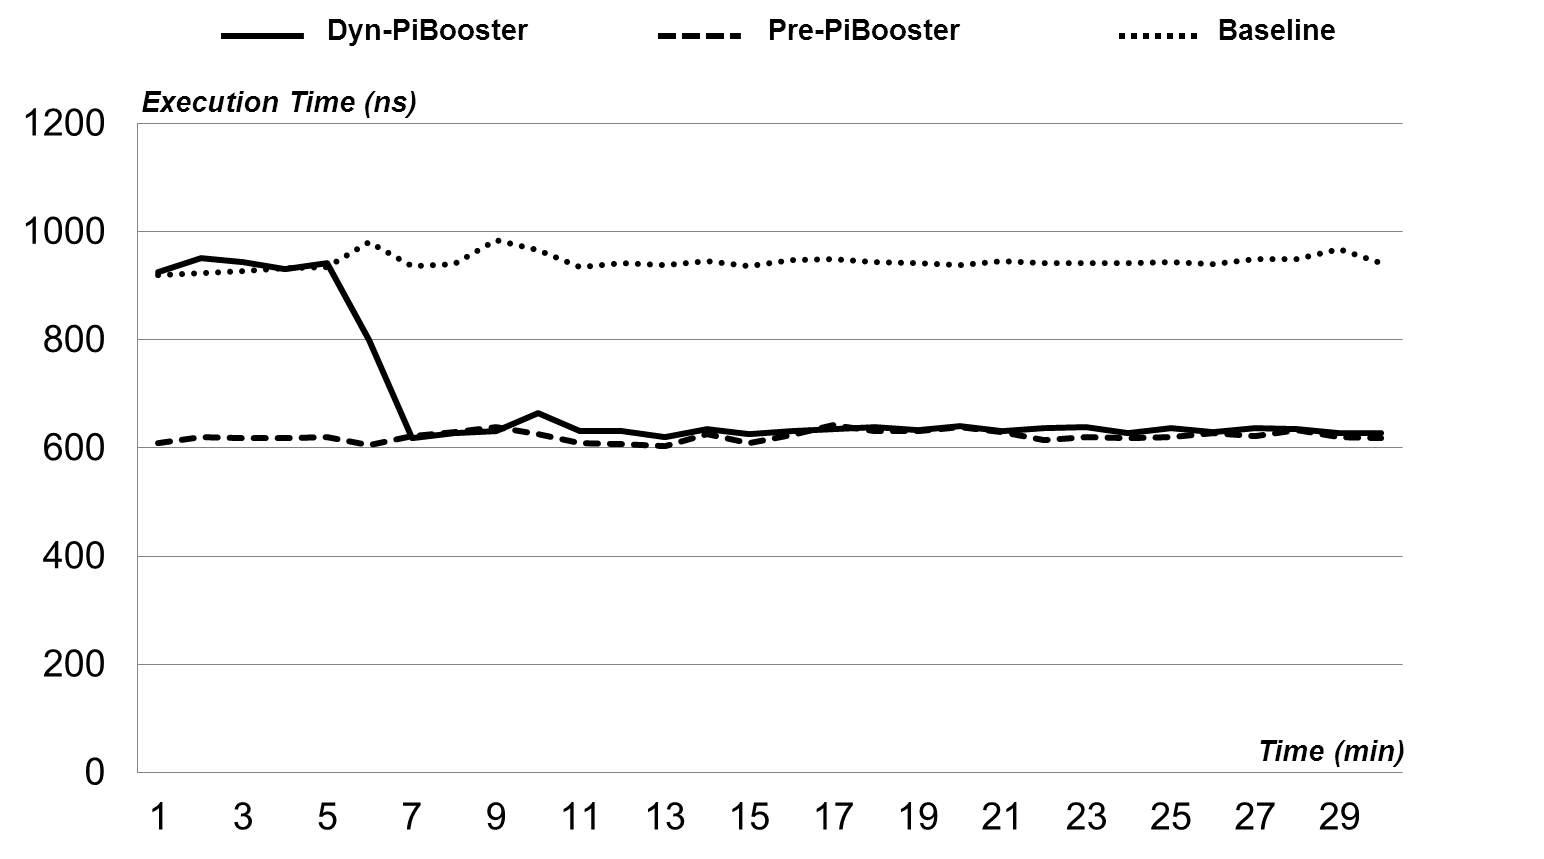
\includegraphics[width=0.5\textwidth]{image/micro/PGDalloc.png}}
%\hspace{1in}
%\subfigure[PGD Free]{
%\label{fig:subfig:b}
%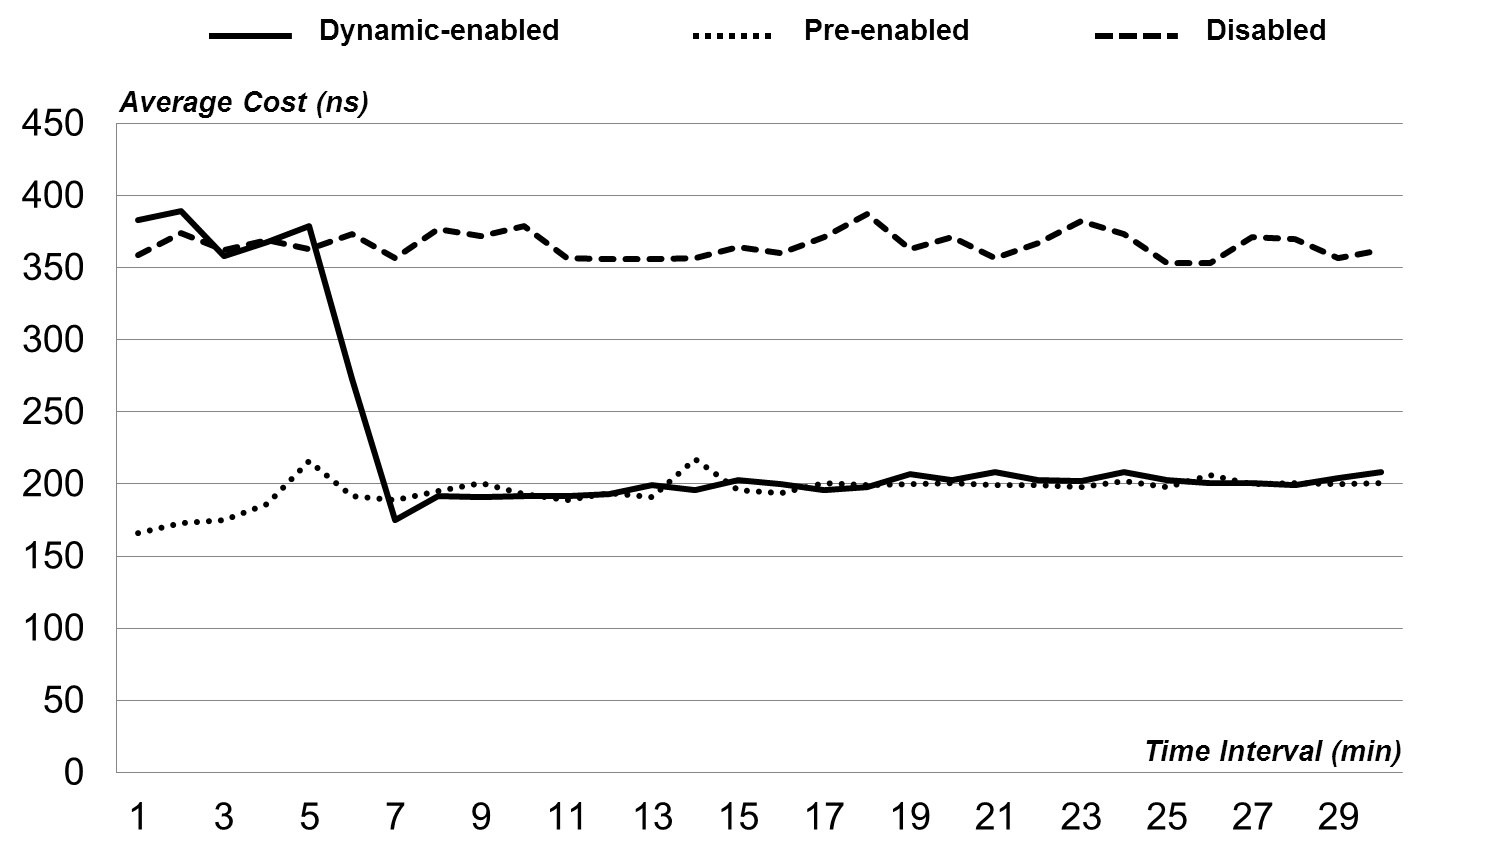
\includegraphics[width=0.5\textwidth]{image/micro/PGDfree.png}}
%\caption{Both page-table cache groups costs much less CPU cycles}
%\label{fig:PGDtime} %% label for entire figure
%\end{figure*}

\begin{figure*}[t!]
    \centering
    \begin{subfigure}[t]{0.5\textwidth}
        \centering
        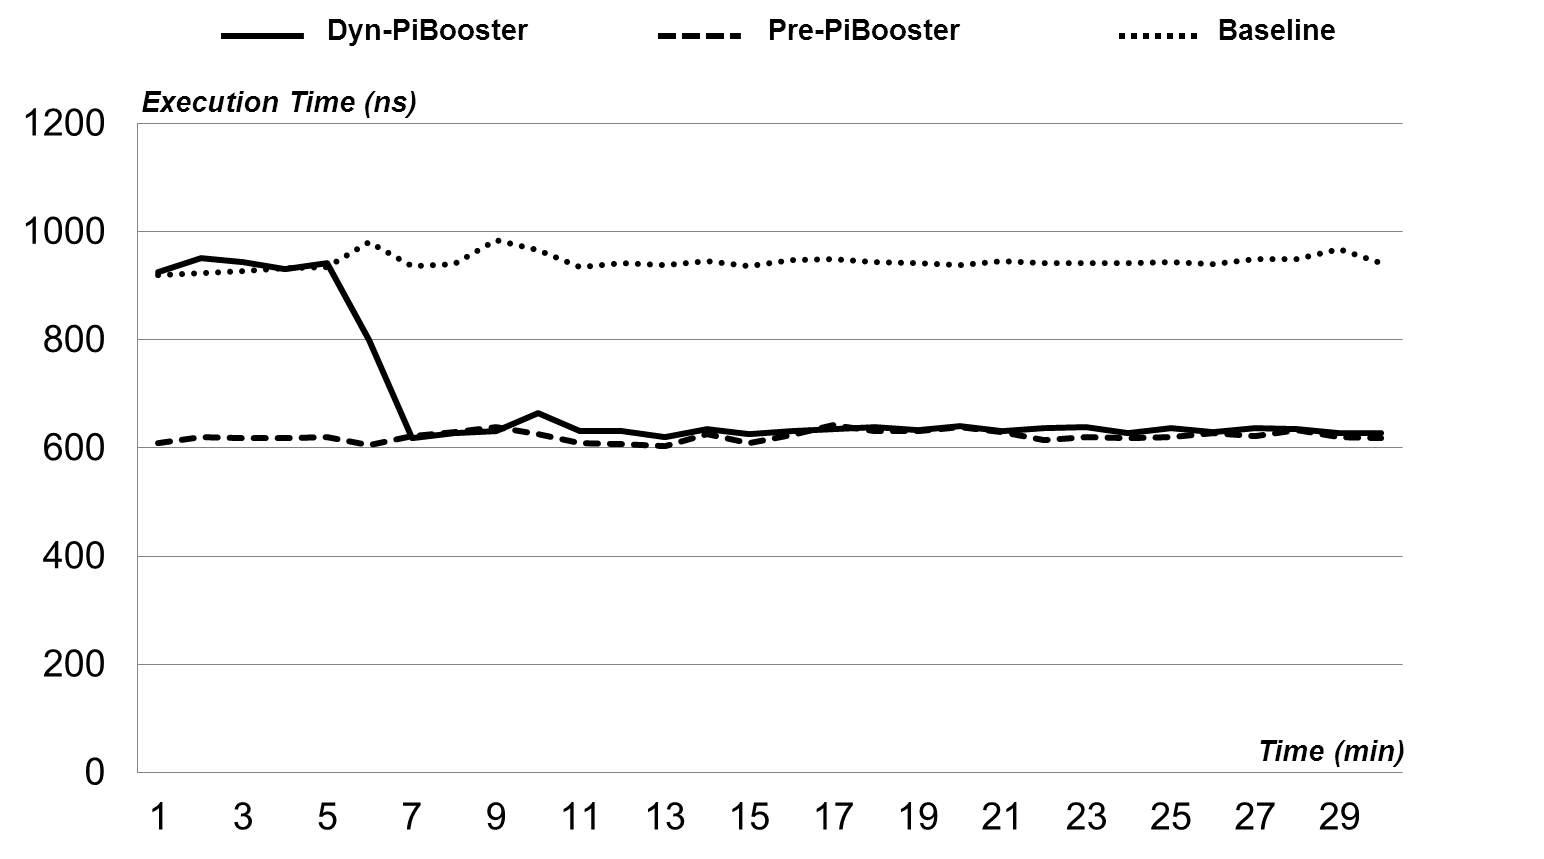
\includegraphics[height=2.0in]{image/micro/PGDalloc.png}
        \caption{PGD Alloc}
        \label{fig:subfig:a}
    \end{subfigure}%
    ~
    \begin{subfigure}[t]{0.5\textwidth}
        \centering
        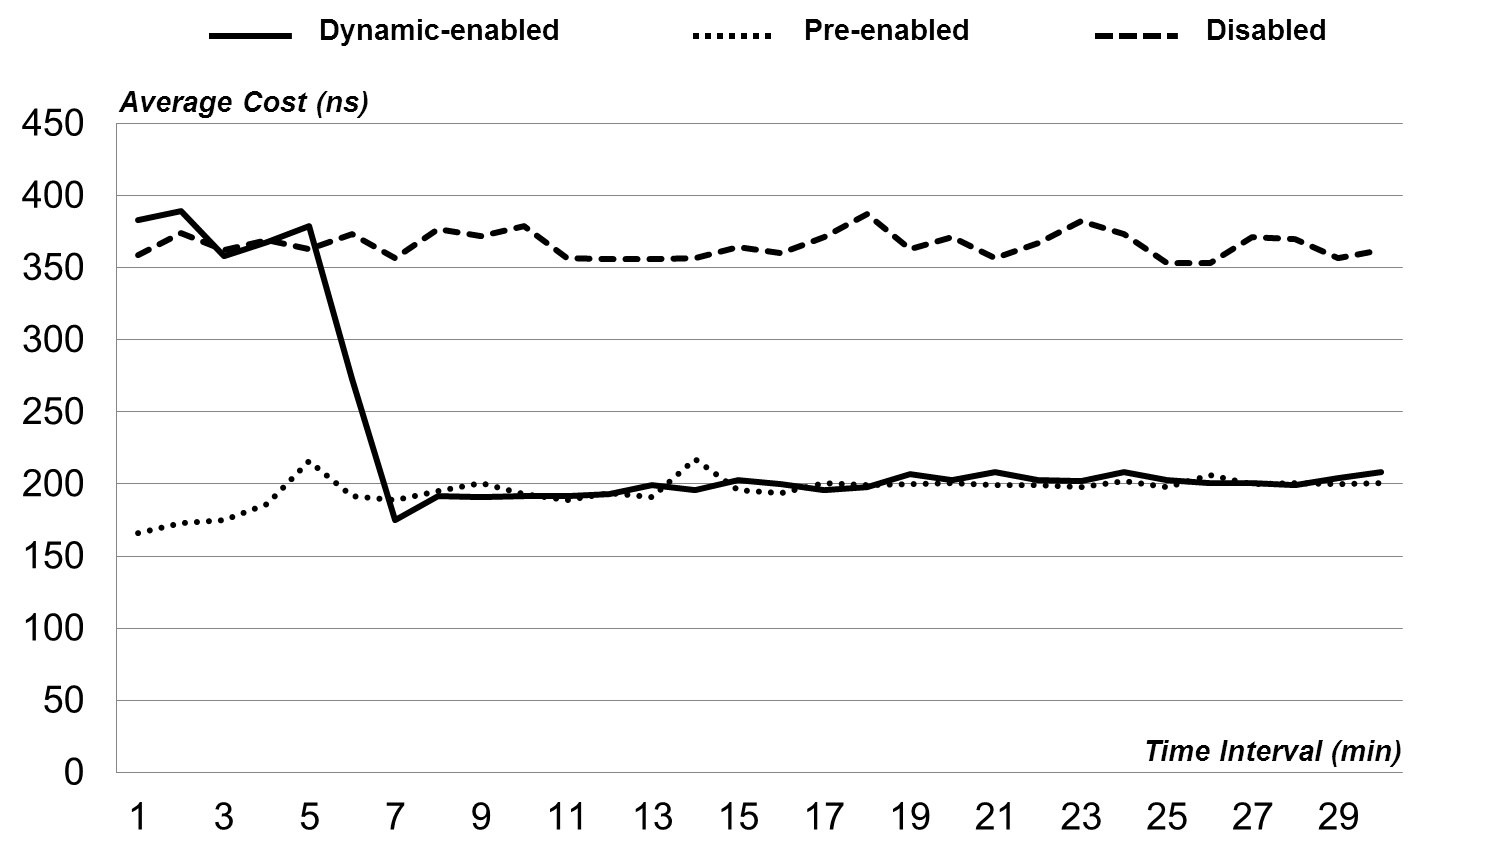
\includegraphics[height=2.0in]{image/micro/PGDfree.png}
        \caption{PGD Free}
        \label{fig:subfig:b}
    \end{subfigure}
    \caption{When the cache is enabled, both functions of PGD Alloc and PGD Free costs much less CPU cycles.}
    \label{fig:PGDtime}
\end{figure*}

\begin{figure*}[t!]
    \centering
    \begin{subfigure}[t]{0.5\textwidth}
        \centering
        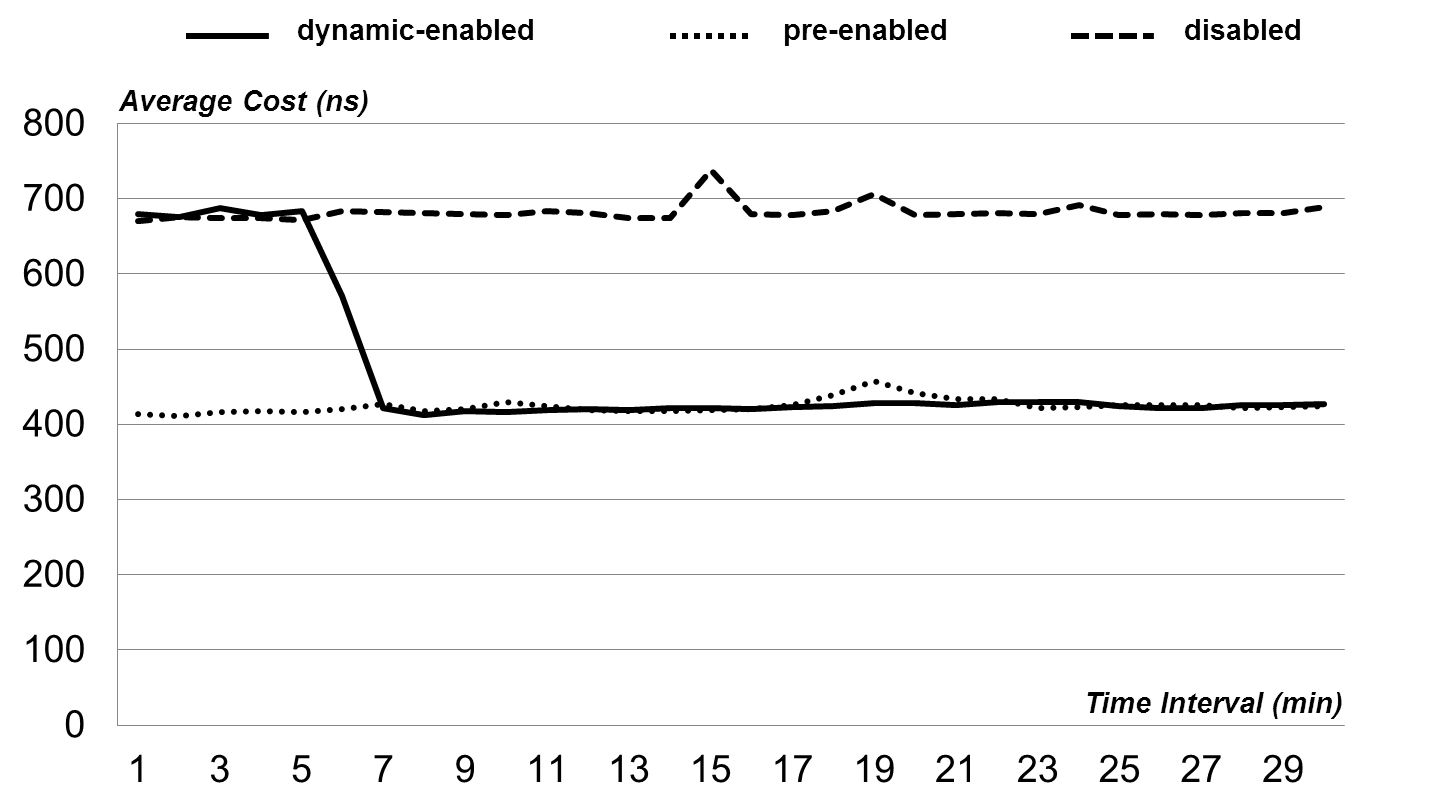
\includegraphics[height=2.0in]{image/micro/PMDalloc.png}
        \caption{PMD Alloc}
        \label{fig:subfig:a}
    \end{subfigure}%
    ~
    \begin{subfigure}[t]{0.5\textwidth}
        \centering
        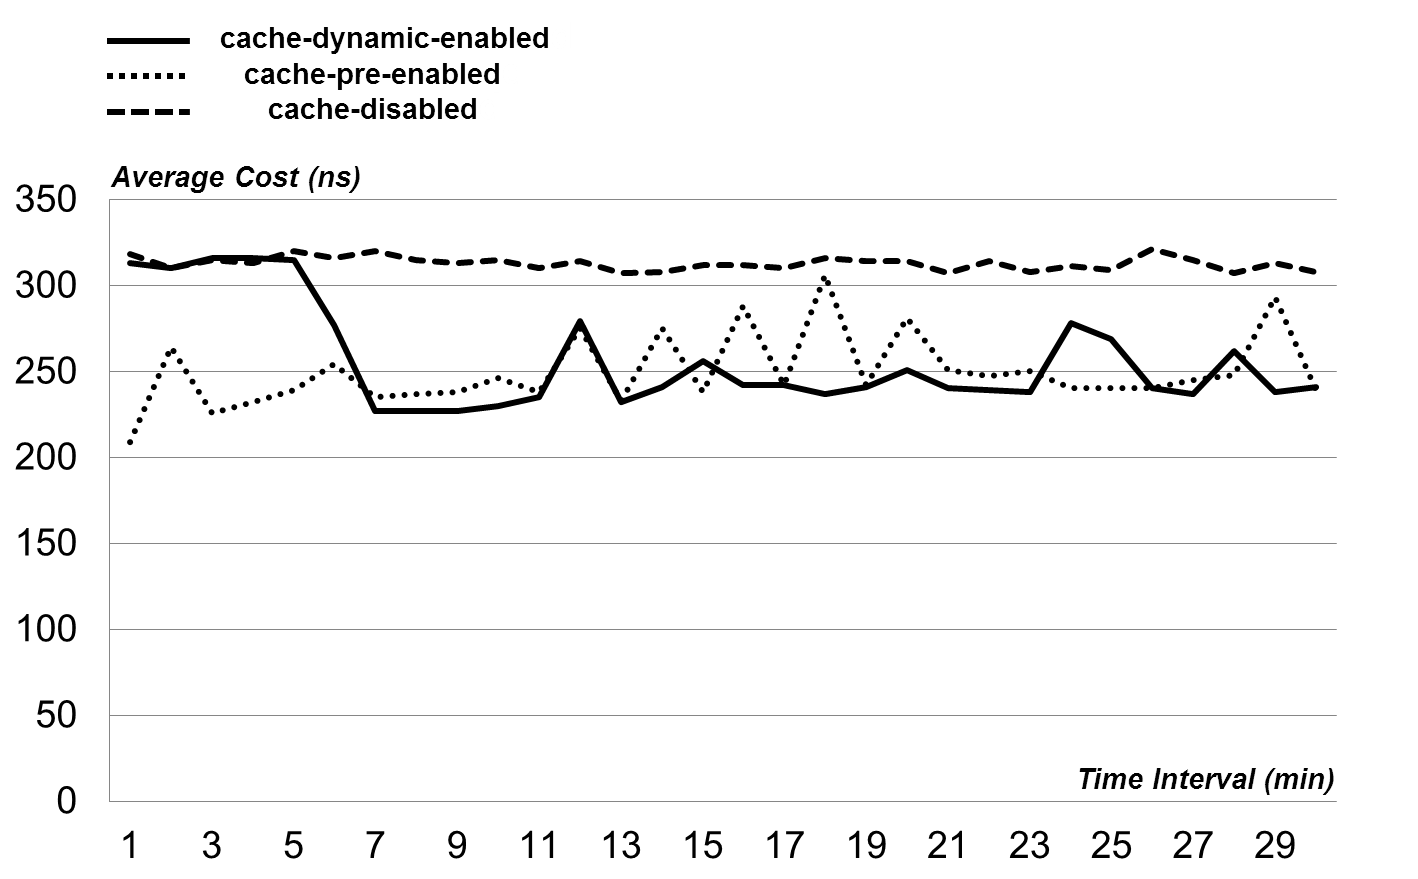
\includegraphics[height=2.0in]{image/micro/PMDfree.png}
        \caption{PMD Free}
        \label{fig:subfig:b}
    \end{subfigure}
    \caption{When the cache is enabled, both functions of PMD Alloc and PMD Free costs much less CPU cycles.}
    \label{fig:PMDtime}
\end{figure*}

\begin{figure*}[t!]
    \centering
    \begin{subfigure}[t]{0.5\textwidth}
        \centering
        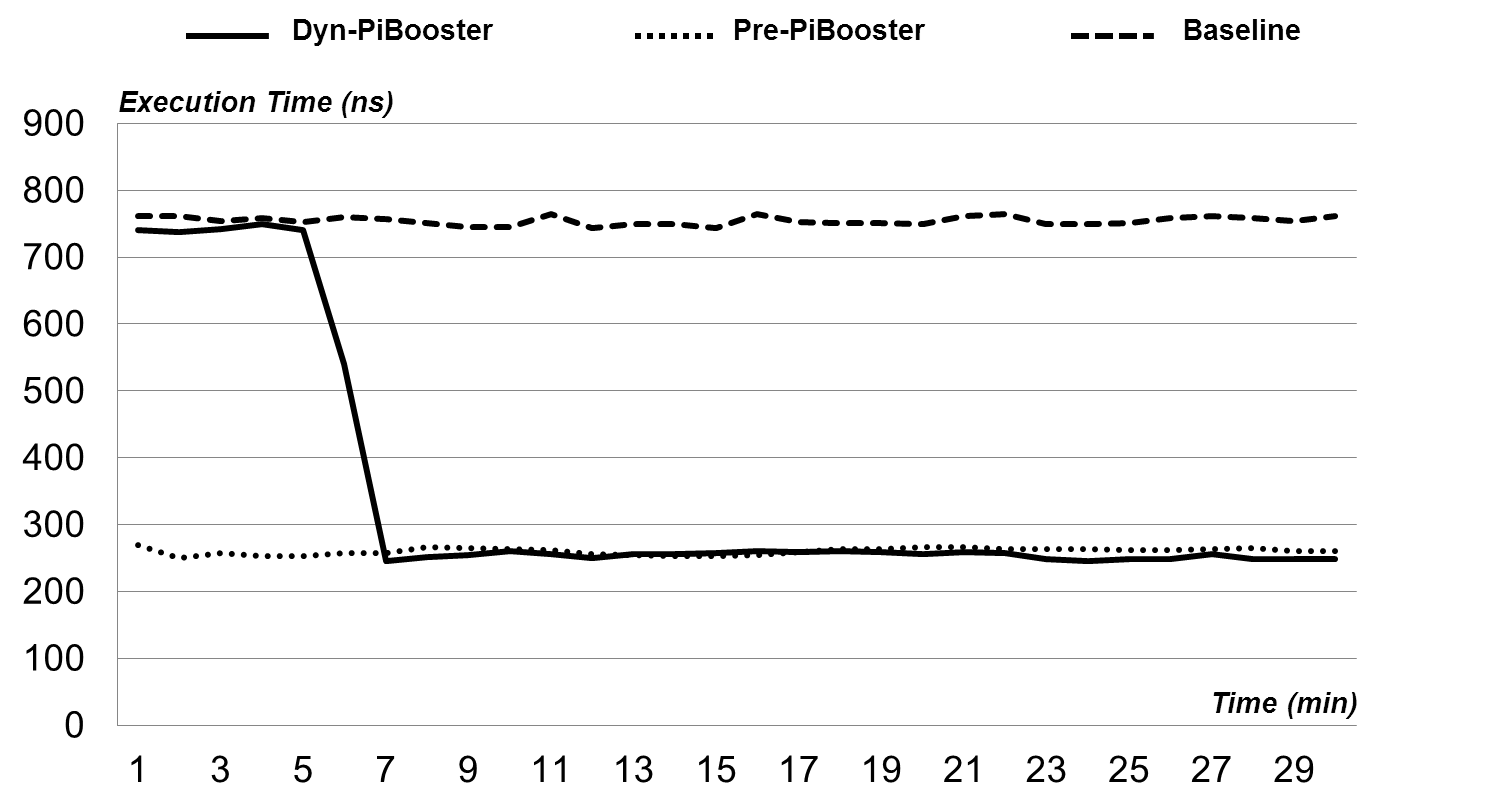
\includegraphics[height=2.0in]{image/micro/PTEalloc.png}
        \caption{PTE Alloc}
        \label{fig:subfig:a}
    \end{subfigure}%
    ~
    \begin{subfigure}[t]{0.5\textwidth}
        \centering
        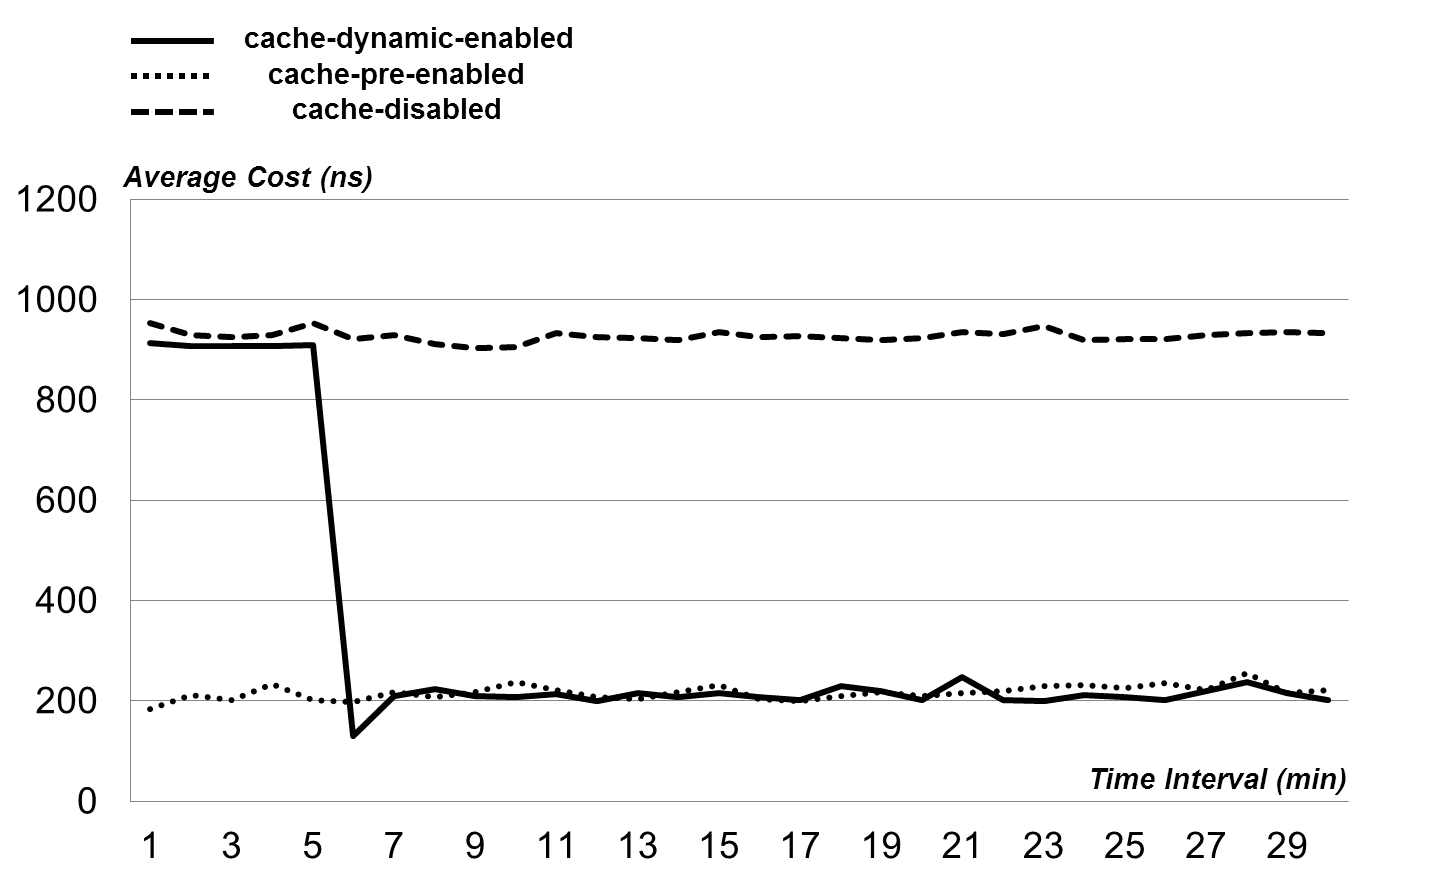
\includegraphics[height=2.0in]{image/micro/PTEfree.png}
        \caption{PTE Free}
        \label{fig:subfig:b}
    \end{subfigure}
    \caption{When the cache is enabled, both functions of PTE Alloc and PTE Free costs much less CPU cycles.}
    \label{fig:PTEtime}
\end{figure*}

%\begin{figure}
%\centering
%\subfigure[PGD]{
%\label{fig:subfig:a}
%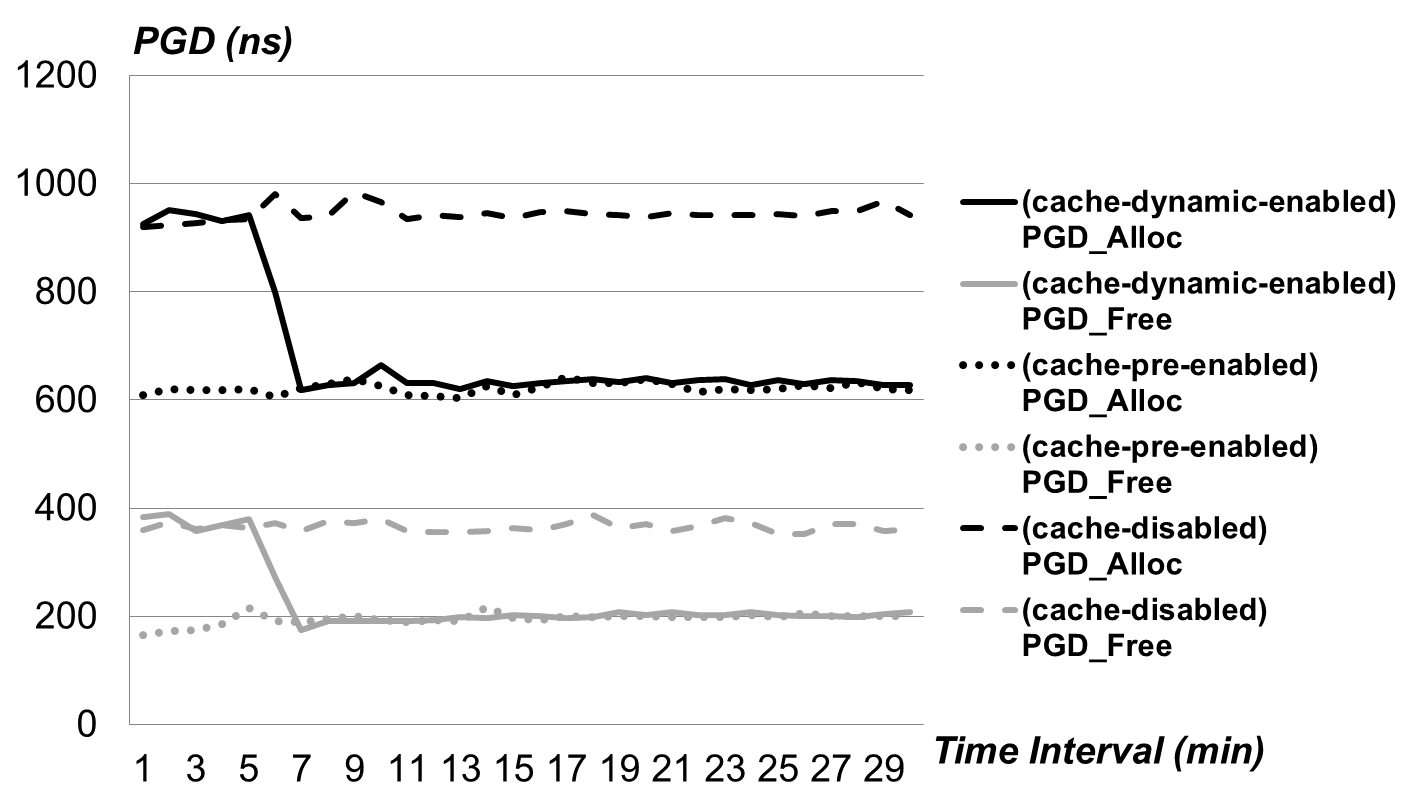
\includegraphics[width=0.5\textwidth]{image/micro/PGDtime.png}}
%\hspace{1in}
%\subfigure[PMD]{
%\label{fig:subfig:b}
%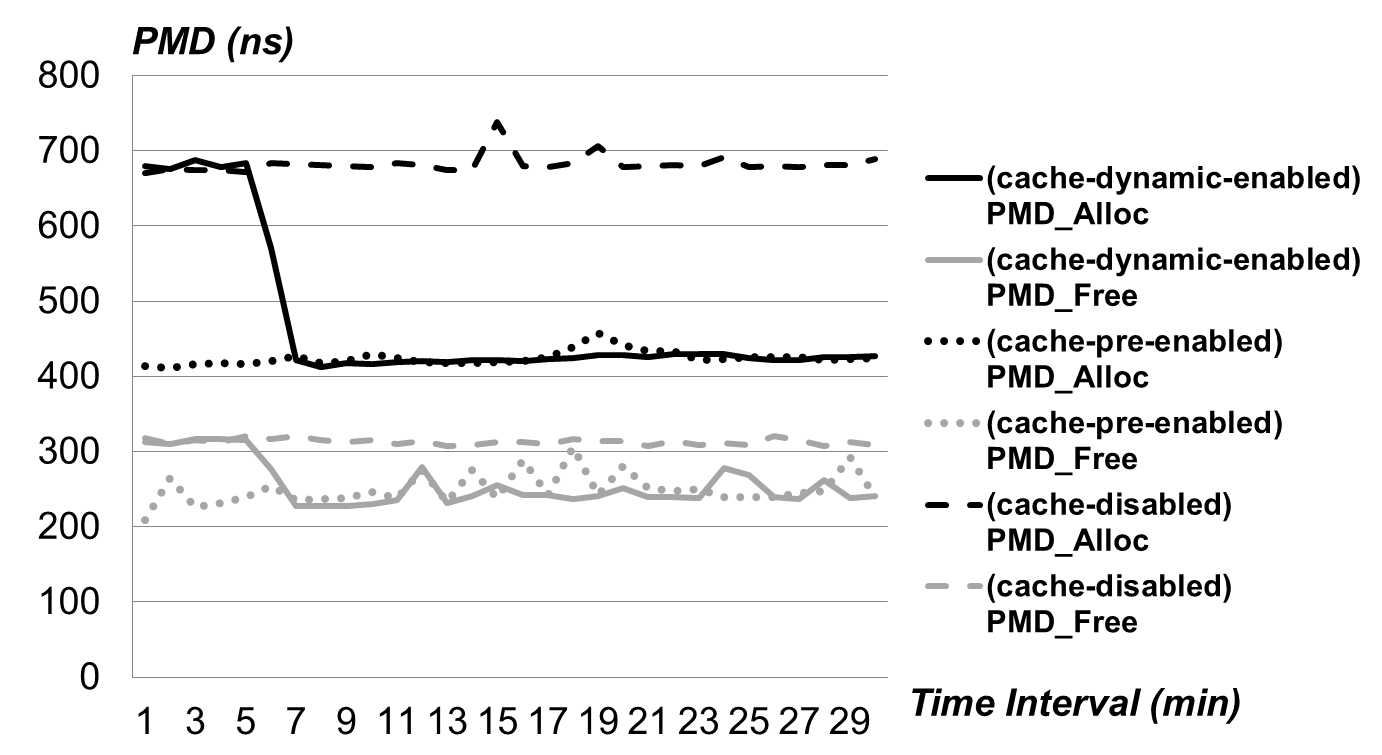
\includegraphics[width=0.5\textwidth]{image/micro/PMDtime.png}}
%\hspace{1in}
%\subfigure[PTE]{
%\label{fig:subfig:c}
%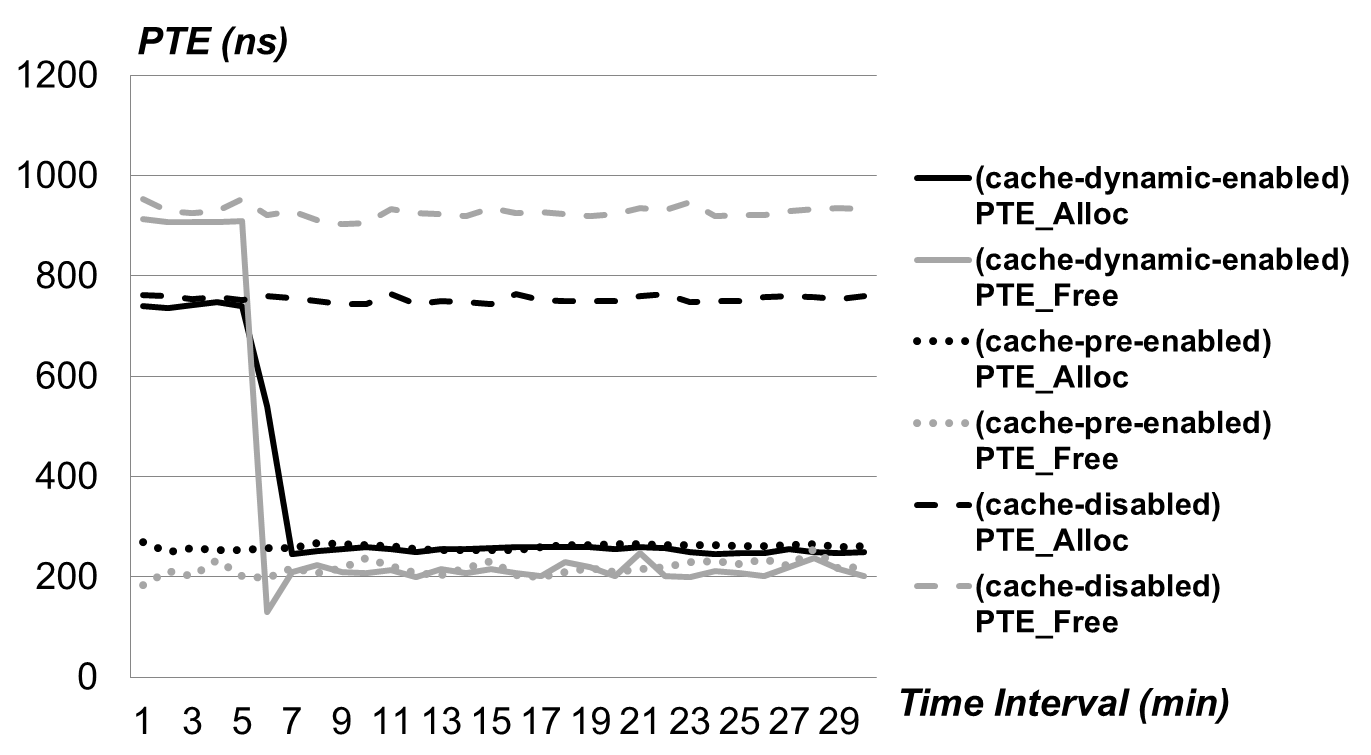
\includegraphics[width=0.5\textwidth]{image/micro/PTEtime.png}}
%\caption{CPU Usage for Each Level of Page Table}
%\label{fig:PGtime} %% label for entire figure
%\end{figure}

Now let’s move to CPU usage that each group will take up. Specifically, each level of page table has its allocation functions and free functions, e.g., pgd\_alloc() and pgd\_free() and the execution time that every related function is calculated per minute. As a result, in Figure \ref{fig:PGDtime}, allocation and free functions in three levels of page tables in the cache-pre-enabled group consumes 45.1\% less and 70.9\% less CPU time in nanoseconds, respectively, compared with that of the cache-disabled group, indicating that a process interacting with the pool has an advantage in saving time over one interacting with the buddy system.

%\begin{figure}
%\centering
%\subfigure[PGD]{
%\label{fig:subfig:a}
%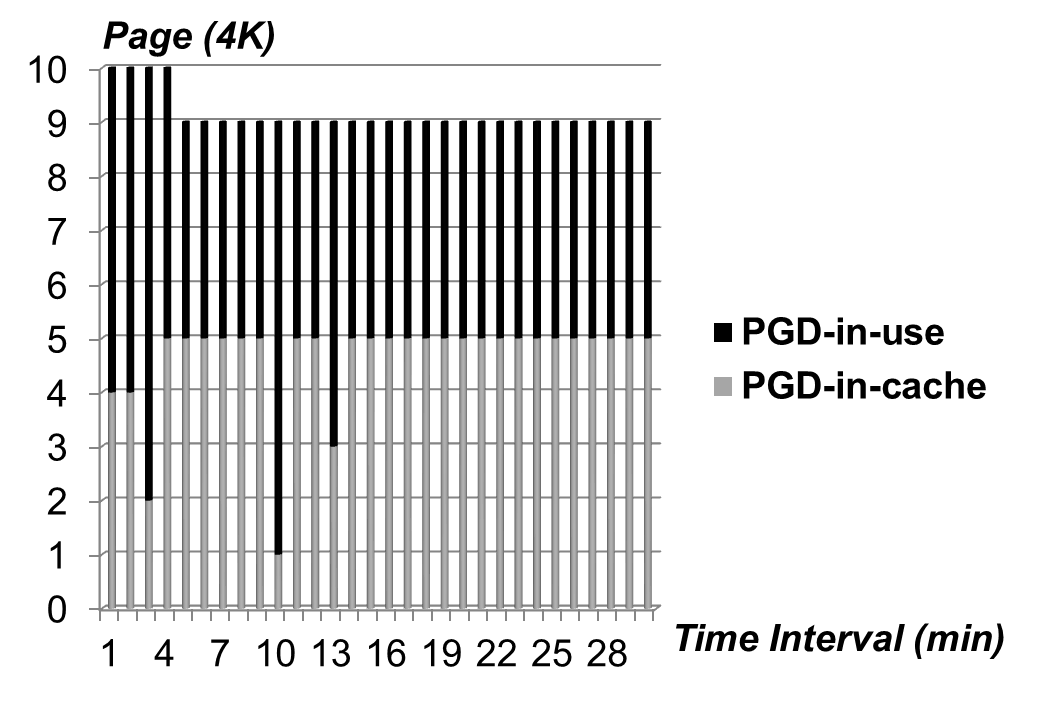
\includegraphics[width=0.5\textwidth]{image/micro/pre_PGDpool.png}}
%\hspace{1in}
%\subfigure[PMD]{
%\label{fig:subfig:b}
%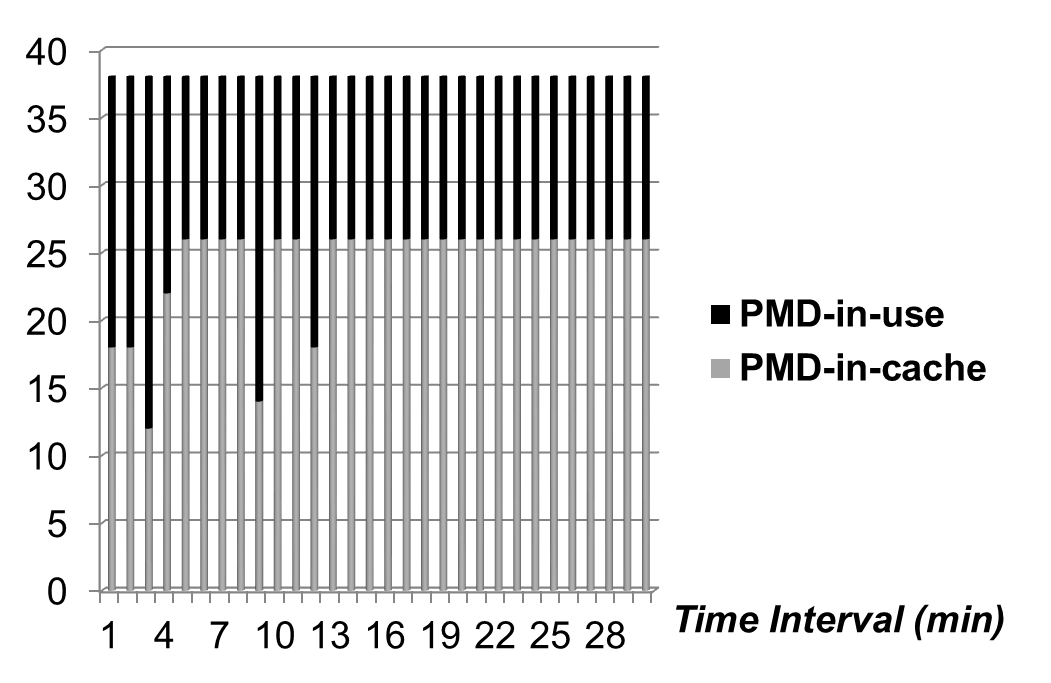
\includegraphics[width=0.5\textwidth]{image/micro/pre_PMDpool.png}}
%\hspace{1in}
%\subfigure[PTE]{
%\label{fig:subfig:c}
%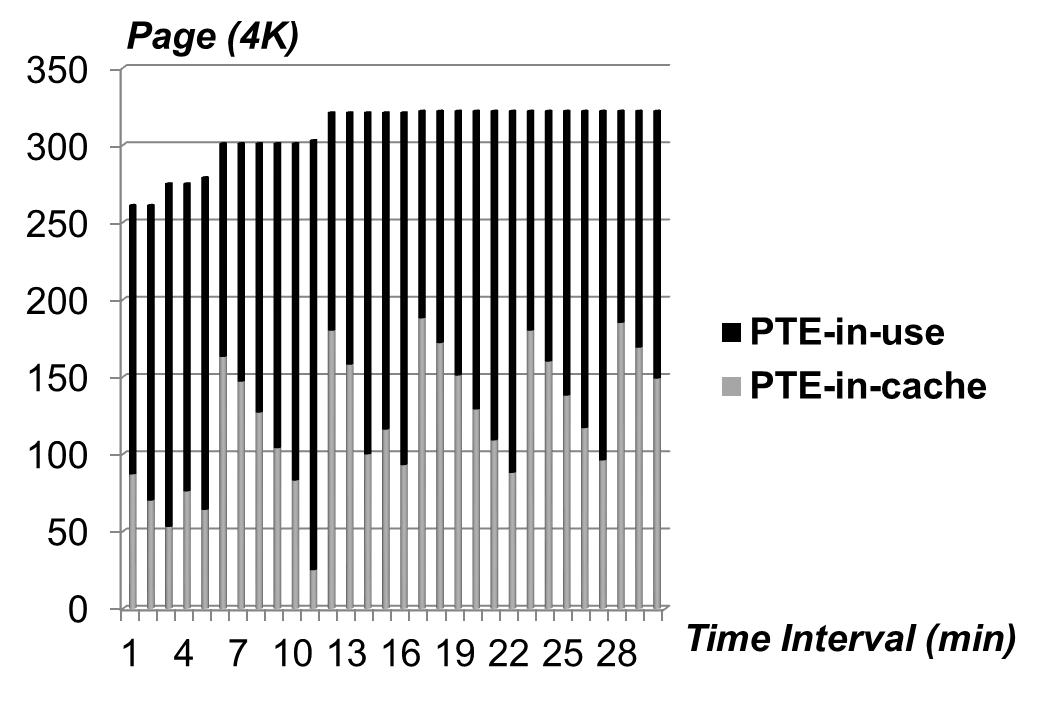
\includegraphics[width=0.5\textwidth]{image/micro/pre_PTEpool.png}}
%\caption{Cache Pools Size for Cache-Pre-Enabled Group}
%\label{fig:prePGpool} %% label for entire figure
%\end{figure}

\begin{table}[!ht]
\footnotesize
\begin{center}
\begin{tabular}{|l|l|l|}
\hline
{\textbf{Page-Table Type}} & {\textbf{Cache (Page \#)}} & {\textbf{Page Table (Page \#)}} \\ \hline
%PGD & $5$  & $4$   & $>1:1$ \\ \hline
%PMD & $26$ & $12$   & $>2:1$ \\ \hline
%PTE & $145$ & $177$ & $<1:1$ \\ \hline
%Total & $176$ & $193$ & $<1:1$ \\ \hline
PGD & $5$  & $4$ \\ \hline
PMD & $26$ & $12$ \\ \hline
PTE & $145$ & $177$ \\ \hline
Total & $176$ & $193$ \\ \hline
\end{tabular}
\end{center}
\caption{When cache is pre-enabled, the ratio between the total pages in cache and the total pages as page tables is approximately equal to 1:1, which indicates that the cache mechanism takes up a small memory percentage of the stress tool.}
\label{tab:prePGpool}
\end{table}

Besides CPU usage, the algorithm is evaluated in the aspect of memory size since three levels of cache pools have been built to support a fast process creation/termination. Cache pools in the cache-pre-enabled group from Figure \ref{tab:prePGpool} takes up $250$ pages(i.e., ($1000$K $=$ $250 * 4K$) $<$ $1$M) at most in the long time run, only 0.35 percentage of the tool's consumption, which is an insignificant usage and reaches a satisfying tradeoff between CPU time costs and space size.

But what if the memory percentage is too high? it is necessary to free pages from the cache pool to the buddy system. Pages in pool will be freed if $1$) a proportion between pages in use and in pool, and $2$) a total number of pages in use and in pool are greater. And data from group of cache-pre-enabled by default is referred to quantify the proportion and the total number. Actually, users can modify the two factors to adjust the cache pool size through an interface. On top of that, page number beyond the proportion is freed, stated in an equation below: $\Delta$num\_to\_free $=$ num\_in\_pool $-$ num\_in\_use.

Since pre-enabling the cache is not flexible enough, we also provide another interface for users to activate the cache mechanism in an on-demand way. For instance, system has been in a busy setting for a while and then cache is enabled manually. Users may make use of this feature to better improve system performance dynamically.

Next, in a group of cache-dynamic-enabled, cache is enabled when IOTLB-flush becomes stable while the freeing mechanism is added so as to check if this group behaves like the cache-pre-enabled group, i.e., cache-dynamic-enabled group could achieve a stable and low enough level in certain aspects, namely, frequency of IOTLB-flush, CPU usage as well as memory size, and it reaches to the level quickly.

%\begin{figure}
%\centering
%\subfigure[PGD]{
%\label{fig:subfig:a}
%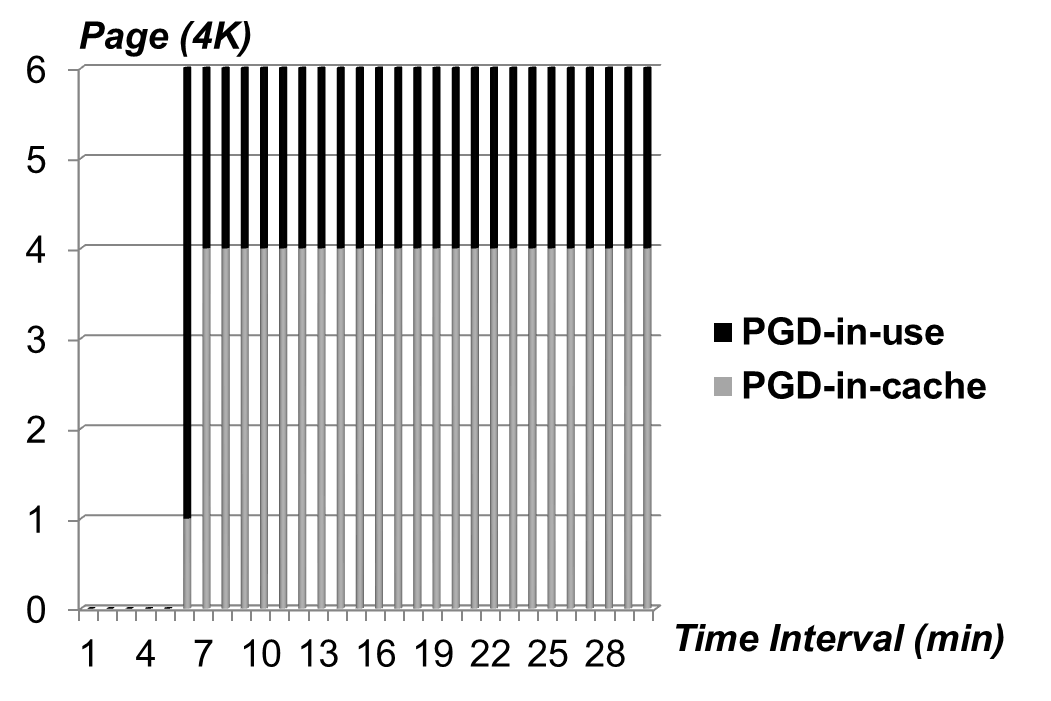
\includegraphics[width=0.5\textwidth]{image/micro/dyn_PGDpool.png}}
%\hspace{1in}
%\subfigure[PMD]{
%\label{fig:subfig:b}
%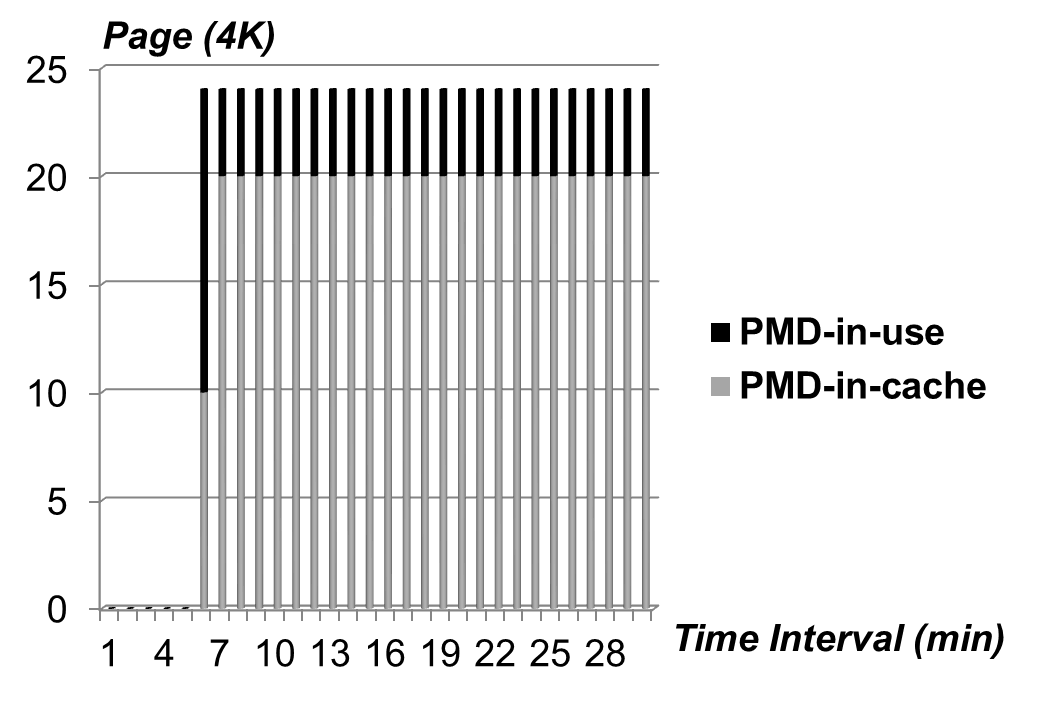
\includegraphics[width=0.5\textwidth]{image/micro/dyn_PMDpool.png}}
%\hspace{1in}
%\subfigure[PTE]{
%\label{fig:subfig:c}
%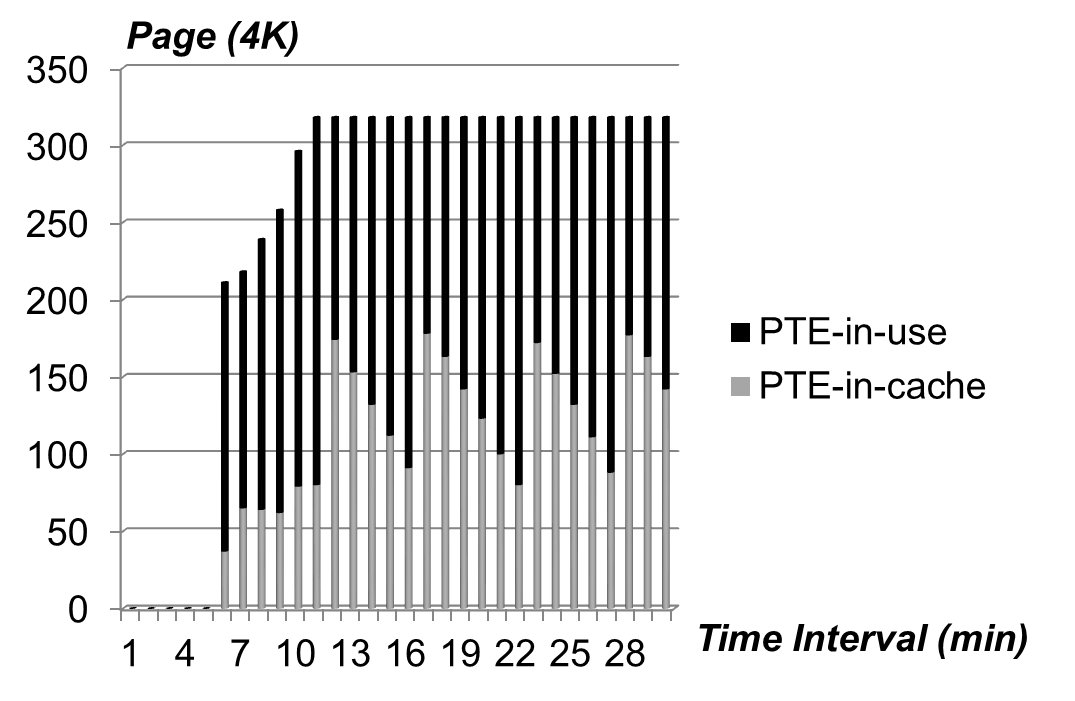
\includegraphics[width=0.5\textwidth]{image/micro/dyn_PTEpool.png}}
%\caption{Cache Pools Size for Cache-Dynamic-Enabled Group}
%\label{fig:dynPGpool} %% label for entire figure
%\end{figure}

\begin{table}[!ht]
\footnotesize
\begin{center}
\begin{tabular}{|l|l|l|}
\hline
{\textbf{Page-Table Type}} & {\textbf{Cache (Page \#)}} & {\textbf{Page Table (Page \#)}} \\ \hline
%PGD & $4$  & $2$   & $2:1$ \\ \hline
%PMD & $20$ & $4$   & $5:1$ \\ \hline
%PTE & $136$ & $182$ & $<1:1$ \\ \hline
%Total & $160$ & $188$ & $<1:1$ \\ \hline
PGD & $4$  & $2$ \\ \hline
PMD & $20$ & $4$  \\ \hline
PTE & $136$ & $182$ \\ \hline
Total & $160$ & $188$ \\ \hline
\end{tabular}
\end{center}
\caption{When cache is dynamically enabled, the pages in cache is effectively freed, while the ratio between the total pages in cache and the total pages as page tables is also approximately equal to 1:1, indicating that the feature of dynamic enabling cache efficiently consumes memory as the cache-pre-enabled group.}
\label{tab:dynPGpool}
\end{table}

From figure \ref{fig:iotlbflush} and \ref{fig:PGtime}, both frequency of IOTLB-flush and CPU usage in this group have a very similar trend with that of the cache-disabled group in the first five minutes, but reduces to zero quickly and stays stable, much like that of the cache-pre-enabled group. In addition, memory size that the cache-dynamic-enabled group in table \ref{tab:dynPGpool} takes up is only $210$ pages at most, also consuming a small percentage. And it is reasonable that the cache-dynamic-enabled group has less pages in the pool since a certain amount of page tables has been freed to the buddy system before the cache pool is put to use.

Also note that the expected results in group of cache-dynamic-enabled is obtained after sever trials by slightly modifying default values of the proportion and the total number. Since these two factors heavily relies on a specific scenario, they may not work for all. How to decide the factors is further discussed in future work.

\subsection{Macro-Benchmarks}

Different micro tests have shown optimizations in three aspects for the algorithm while macro-benchmarks are made use of to evaluate its effects on overall system performance. Since cache-disabled group does not apply to real case, macro tests are conducted in two groups, i.e., cache-disabled group and cache-dynamic-enabled group.

\begin{figure}[htp]
\centering
%\includegraphics[scale=0.55]{image/iotlbflush.png} \\
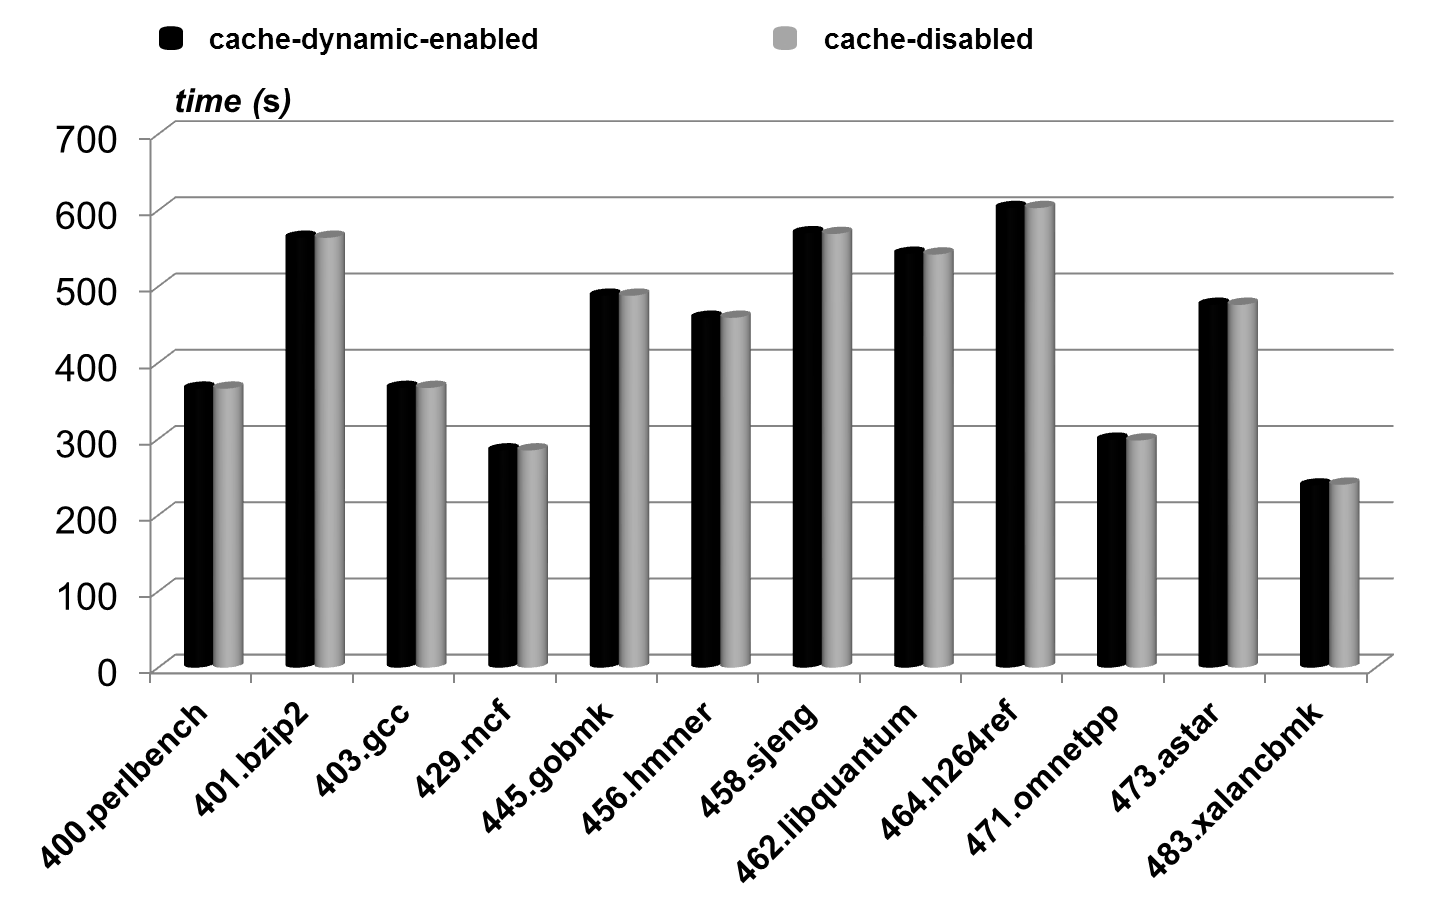
\includegraphics[width=0.5\textwidth]{image/macro/spec.png} \\
\caption{System performance produced by \name is almost the same as usual.}
\label{fig:spec}
\end{figure}

SPECint\_2006v1.2 has $12$ benchmarks in total and they are all invoked with EXAMPLE-linux64-ia32-gcc43+.cfg for integer computation, results of which produce Figure \ref{fig:spec}. 483.xalancbmk in cache-dynamic-enabled group costs $239$ seconds, 0.42\% less
than that of the cache-disabled group and this is the biggest difference among all benchmarks. As a result, little difference between the two groups exists, which indicates that the algorithm does not have any bad effect on system performance.

\begin{figure}[htp]
\centering
%\includegraphics[scale=0.55]{image/iotlbflush.png} \\
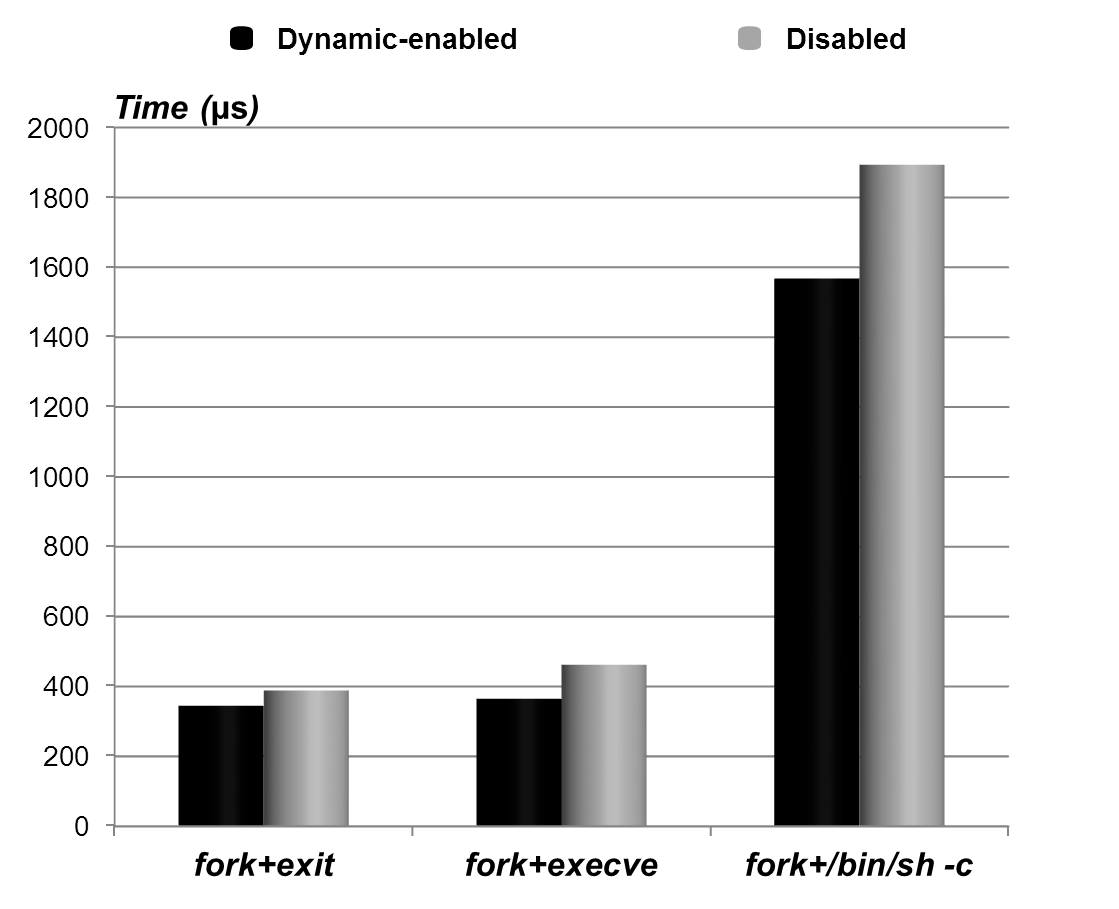
\includegraphics[width=0.5\textwidth]{image/macro/lmbench.png} \\
\caption{Every process costs less CPU time when the cache is enabled.}
\label{fig:lmbench}
\end{figure}

Lmbench is used to measure CPU time that processes cost (i.e., fork+exit, fork+execve, fork+/bin/sh -c), shown in Figure \ref{fig:lmbench}. The configuration parameters are selected by default, except parameters of processor MHz, a range of memory and mail result, since CPU mhz of our test machine is $3.2$ GHz rather than the default one, memory range uses $1024$ MB to save time that Lmbench-run costs and we need no results mailed. As can be seen from the figures, command of fork+exit in cache-dynamic-enabled group costs $344$ microseconds, 11\% less than that of the cache-disabled group. and other two commands also perform well. Undoubtedly, the algorithm has reduced CPU cycles.

%\begin{figure}[htp]
%\centering
%\includegraphics[scale=0.55]{image/iotlbflush.png} \\
%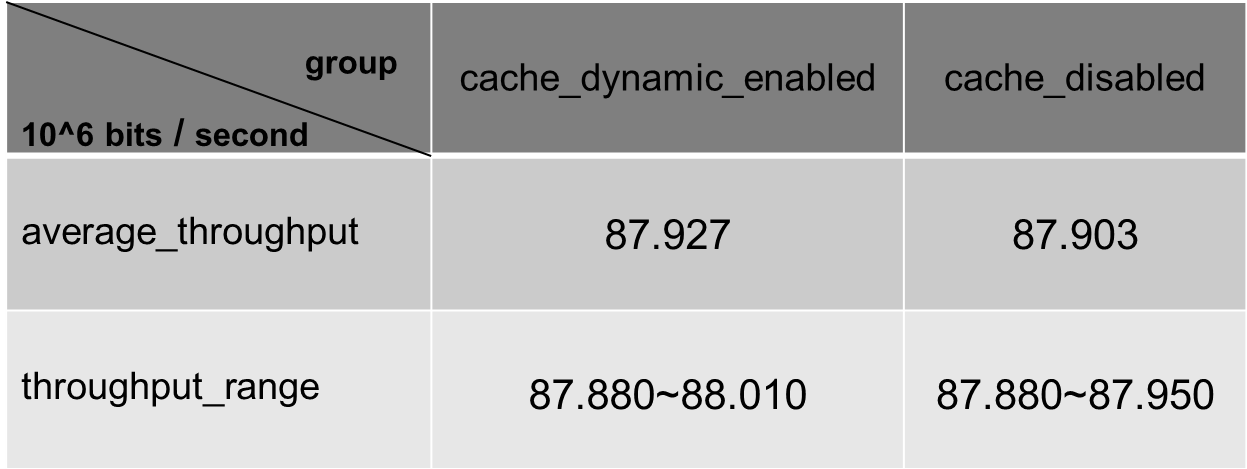
\includegraphics[width=0.5\textwidth]{image/macro/netperf.png} \\
%\caption{Netperf}
%\label{fig:netperf}
%\end{figure}
%|p{1.7cm}|p{1.8cm}|p{1.7cm}

\begin{table}[!ht]
\footnotesize
\begin{center}
\begin{tabular}{|l|l|l|}
\hline
{\textbf{Throughput ($10^6$ bits per second)}} & {\textbf{dynamic-enabled}} & {\textbf{disabled}}    \\ \hline
Average Throughput &  $87.927$ & $87.903$ \\ \hline
Range of Throughput & $87.880-88.010$ & $87.880-87.950$ \\ \hline
\end{tabular}
\end{center}
\caption{When the cache is enabled, the upper limit of the throughput range is improved by 0.06\% while the average throughput of 30 runs is improved by 0.02\%. }
\label{tab:netperf}
\end{table}

As for I/O performance, we use netperf to evaluate the performance of network-intensive workloads. To overcome the adverse effect caused by real network jitter, we physically connect the testing machine directly to a tester machine by a network cable, and then the tester machine as a client measures a network throughput by sending a bulk of TCP packets to the testing machine being a server. Specifically, the client connects to the tested server by building a single TCP connection. Test type is TCP\_STREAM, sending buffer size is $16KB$ and connection lasts $60$ seconds. On top of that, the TCP\_STREAM test of netperf is conducted for $30$ runs to obtain an average throughput. Throughput in cache-dynamic-enabled group is $87.93 \times 10^6$ bits per second, 0.02\% more than that of the cache-disabled group, shown in figure\ref{tab:netperf}, and this makes no difference.
Seemingly, the results indicate that the algorithm has no contribution to the performance improvement, contradicting with the results from micro experiments.

Actually, Nadav Amit [xxx] demonstrates that the virtual I/O memory map and unmap operations consume more CPU cycles than  that of the corresponding DMA transaction so that the IOTLB has not been observed to be a bottleneck under regular circumstances. Thus, only when the cost of frequent mapping and unmapping of IOMMU buffers is sufficiently reduced, the guest physical address resolution mechanism becomes the main bottleneck. Furthermore, he proposes the so-called pseudo pass-through mode and utilizes a high-speed I/O device (i.e., Intel’s I/O Acceleration Technology) to reduce time required by DMA map and unmap operations so that IOTLB becomes the dominant factor. As a result, it is quite reasonable that netperf results with/without the algorithm are almost the same.








